\documentclass[12pt, titlepage]{article}

\usepackage{booktabs}
\usepackage{tabularx}
\usepackage{hyperref}
\usepackage{graphicx}
\usepackage{subcaption}
\usepackage{float}
\hypersetup{
    colorlinks,
    citecolor=black,
    filecolor=black,
    linkcolor=red,
    urlcolor=blue
}
\usepackage[round]{natbib}

\input{../Comments.text}
\input{../Common.text}

\begin{document}

\title{Verification and Validation Report: \progname} 
\author{\authname}
\date{\today}
	
\maketitle

\pagenumbering{roman}

\section{Revision History}

\begin{tabularx}{\textwidth}{p{3cm}p{2cm}X}
\toprule {\bf Date} & {\bf Version} & {\bf Notes}\\
\midrule
April 21, 2026 & 1.0 & Initial upload\\
% Date 2 & 1.1 & Notes\\
\bottomrule
\end{tabularx}

~\newpage

\section{Symbols, Abbreviations and Acronyms}

See SRS Documentation at \href{https://krozix-2026.github.io/cas741-speech-trf/SRS/SRS.pdf}{SRS}.

% \renewcommand{\arraystretch}{1.2}
% \begin{tabular}{l l} 
%   \toprule		
%   \textbf{symbol} & \textbf{description}\\
%   \midrule 
%   T & Test\\
%   \bottomrule
% \end{tabular}\\

% \wss{symbols, abbreviations or acronyms -- you can reference the SRS tables if needed}

\newpage

\tableofcontents

\listoftables %if appropriate

\listoffigures %if appropriate

\newpage

\pagenumbering{arabic}

This document summarized the result of the 
\href{https://krozix-2026.github.io/cas741-speech-trf/VnVPlan/VnVPlan.pdf}{VnV Plan}. 
The requirements that were being tested are detailed in the 
\href{https://krozix-2026.github.io/cas741-speech-trf/SRS/SRS.pdf}{SRS}.







\section{Functional Requirements Evaluation}
\label{sec_funcEval}

This section presents the evaluation of the functional requirements of \progname.
The goal of these tests is to verify that each major module satisfies its intended behavior under normal and invalid input conditions.
The evaluation focuses on core data loading, parameter validation, and trained model loading functionality.
Detailed test procedures and source files are provided in the referenced unit and integration test files.

\subsection{Audio Data Module Test}

These test cases are designed to evaluate the basic functionality of the Audio Data Module.
They verify that the LibriSpeech manifest can be found and read correctly, that the dataset is not empty, that feature files referenced by the manifest can be loaded, and that the cochleagram feature arrays have the expected shape.
The tests also check that subset filtering, sample limiting, and batch collation behave as intended, and that invalid or missing feature files are handled properly.

\textbf{Result:} All test cases are passed.

Test file: \href{https://github.com/Krozix-2026/cas741-speech-trf/blob/main/src/test/test_librispeech_aligned_words_unit.py}{test\_librispeech\_aligned\_words\_unit.py}, \\ \href{https://github.com/Krozix-2026/cas741-speech-trf/blob/main/src/test/test_librispeech_aligned_words_integration.py}{test\_librispeech\_aligned\_words\_integration.py} [VnV Plan FR-05]

\subsection{MEG Data Module Test}

These test cases are designed to evaluate the basic functionality of the MEG Data Module.
They verify that the Appleseed dataset root path is correct, that the subject folders \texttt{sub-01} to \texttt{sub-12} exist, and that each subject contains a \texttt{meg} directory with readable \texttt{.fif} files.
The tests also check whether the number of \texttt{.fif} files is consistent across subjects and whether the empty-room recording folder contains the required \texttt{.fif} file(s).

\textbf{Result:} All test cases passed.

Test file: \href{https://github.com/Krozix-2026/cas741-speech-trf/blob/main/src/test/test_appleseed_meg_dataset.py}{test\_appleseed\_meg\_dataset.py} [VnV Plan FR-01]

\subsection{Input Parameters Module Test}

These test cases are designed to evaluate the Input Parameters Module.
They verify that configuration enums, local paths, preset training templates, and schema-level validation rules behave correctly.
The tests check that valid input parameters are normalized and accepted, while invalid parameter values, unsupported parameter combinations, and missing required paths are rejected with appropriate errors.
They also confirm that preset configurations generate the expected training setup and that utility functions such as run directory generation and JSON export work correctly.

\textbf{Result:} All test cases passed.

Test file: \href{https://github.com/Krozix-2026/cas741-speech-trf/blob/main/src/test/test_input_parameters_module.py}{test\_input\_parameters\_module.py} [VnV Plan FR-02, FR-03]

\subsection{Trained Model Feature Dimension Test}

These test cases are designed to evaluate whether a trained deep learning model's feature can be loaded correctly into the target network architecture.
They verify that the checkpoint loader can extract model weights from different checkpoint formats, remove unnecessary key prefixes when needed, and load the parameters into the network without crashing, and check the feature dimension.
The tests also check that invalid checkpoint files are rejected properly and that the loaded model can execute a forward pass successfully.

\textbf{Result:} All test cases passed.

Test file: \href{https://github.com/Krozix-2026/cas741-speech-trf/blob/main/src/test/test_model_ckpt_loading.py}{test\_model\_ckpt\_loading.py} [VnV Plan FR-04]



\subsection{Predictor Validation and Alignment Test}

These test cases are designed to evaluate the correctness of the generated predictor files and the behavior of predictor--MEG time alignment.
The integration tests verify that predictor files with the \texttt{.pickle} suffix exist in the expected Appleseed derivatives directory, that required predictor files for a subject can be found, and that these files can be loaded successfully.
They also check that predictor dimensions are correct and that different predictors from the same subject have compatible time axes.

Additional unit tests are designed to evaluate error handling in predictor alignment.
A small synthetic MEG time grid and an incompatible predictor are constructed, and the predictor-alignment function is called to verify that alignment fails with a descriptive error message when the time axis is incompatible.

\textbf{Result:} All test cases passed.

Test file: \href{https://github.com/Krozix-2026/cas741-speech-trf/blob/main/src/test/test_appleseed_predictors.py}{test\_appleseed\_predictors.py}, \href{https://github.com/Krozix-2026/cas741-speech-trf/blob/main/src/test/test_predictor_alignment.py}{test\_predictor\_alignment.py} [VnV Plan FR-06]





\subsection{Predictor Evaluation Protocol Validation Test}

These test cases are designed to evaluate the consistency of protocol metadata across predictors used in the same evaluation setting.
In the test, two predictors are defined in \texttt{pytest}, and one protocol field is intentionally assigned a conflicting value in one predictor.
The evaluation protocol validation function is then called to verify that validation fails with an informative error message listing the conflicting protocol field name or names.
Additional test cases verify that validation succeeds when all protocol fields are consistent across predictors.

This test is included in the Unit Test of the predictor evaluation pipeline, since it verifies protocol consistency checking before model evaluation is performed.
It helps prevent invalid combinations of predictors from being used in the same evaluation setting.

\textbf{Result:} All test cases passed.

Test file: \href{https://github.com/Krozix-2026/cas741-speech-trf/blob/main/src/test/test_predictor_protocol_validation.py}{test\_predictor\_protocol\_validation.py} [VnV Plan FR-07]







\subsection{Encoding Score Invalidity Handling Test}

These test cases are designed to evaluate whether the system correctly rejects invalid or undefined encoding-score computations.
In \texttt{pytest}, small synthetic predictor and response matrices are constructed on the same time grid, and invalid scoring conditions are introduced intentionally.
Examples include inserting a \texttt{NaN} value into the predictor matrix and providing a constant response signal that makes Pearson correlation undefined.
The scoring function is then called to verify that scoring fails with a descriptive error message identifying the specific cause of invalidity, such as non-finite predictor values or undefined correlation due to a constant response signal.

Additional test cases verify related failure conditions, such as constant predictor signals or incompatible time grids in NDVar-based inputs.
Integration tests are also used to confirm that cached Eelbrain scoring outputs do not contain invalid \texttt{NaN} or infinite values.

\textbf{Result:} All test cases passed.

Test file: \href{https://github.com/Krozix-2026/cas741-speech-trf/blob/main/src/test/test_encoding_score_invalidity.py}{test\_encoding\_score\_invalidity.py}, \\  \href{https://github.com/Krozix-2026/cas741-speech-trf/blob/main/src/test/test_eelbrain_cached_scores.py}{test\_eelbrain\_cached\_scores.py} [VnV Plan FR-08]













\section{Nonfunctional Requirements Evaluation}

This section summarizes the evaluation of the nonfunctional requirements of \progname.
The evaluated requirements are usability, maintainability, portability, reproducibility, and performance, as defined in the VnV Plan.

\subsection{Correctness}

Correctness is not evaluated here as a separate nonfunctional requirement.
Instead, correctness is evaluated through the functional requirement tests in Section~\ref{sec_funcEval}.
This subsection is included only to clarify that functional correctness has been addressed separately.

\subsection{Usability}

NFR-01 evaluates whether \progname{} is easy to use for users familiar with speech and MEG analysis. 
The complete workflow of the project was demonstrated in class.
In addition, face-to-face discussions were conducted with users familiar with Eelbrain, including Lizhangwenchi and Yanyu, to evaluate whether the workflow was easy to understand and operate.
All respondents indicated that the workflow was straightforward to use and that the system was easy to extend for future experiments.

The project was also discussed with Professor Brodbeck.
His feedback was that the project was well designed and could be used by future students to conduct experiments, thereby substantially reducing the onboarding cost for new lab members.

\textbf{Result:} Requirement satisfied.

\textbf{Evidence:} In-class demonstration, face-to-face user feedback from Eelbrain users, and discussion feedback from Professor Brodbeck.

\subsection{Maintainability}

NFR-02 evaluates maintainability through the effort required to implement a likely future change.
The project is designed to be extensible.
To support a new deep learning model, the main required modifications are to add a new network file under the \texttt{network} directory and to add the corresponding configuration entries under the \texttt{config} directory.
In particular, modifications to the configuration files require fewer than 10 lines of code in typical cases.

This structure reduces the effort required to extend the system and allows new model variants to be integrated without modifying the rest of the pipeline.
The modular organization therefore supports both maintainability and future experimentation.

\textbf{Result:} Requirement satisfied for the evaluated likely-change scenario.

\textbf{Evidence:} Modular directory structure and observed low-effort configuration changes for adding new model settings.

\subsection{Portability}

NFR-03 evaluates whether the system can be installed and executed across different operating systems. 
Extensive experiments have already been conducted on both Windows and Linux.
At the time of writing, the project has not yet been tested on macOS.
The implementation mainly depends on Python, PyTorch, and CUDA-related software components.
Therefore, the system is expected to run on any platform that provides the required software environment and dependency versions.

Since successful execution has been demonstrated on both Windows and Linux, the project shows partial evidence of portability.
However, full satisfaction of this requirement is deferred until macOS has also been tested.

\textbf{Result:} Partially satisfied.

\textbf{Evidence:} Successful execution on Windows and Linux; macOS evaluation not yet completed.

\subsection{Reproducibility}

NFR-04 evaluates reproducibility through repeat-run consistency under fixed configuration, fixed input data, and fixed random seed. 
For this project, reproducibility should be evaluated at two levels:
(1) deep learning training/testing outputs, and
(2) Eelbrain mTRF analysis outputs.
The same workflow should be executed twice without changing the code version, configuration, input data, or random seed.
The output artifact structure and scalar summary metrics should then be compared.

Table~\ref{tab:reproducibility-results} is used to summarize the reproducibility results.


\begin{table}[ht]
\centering
\caption{Reproducibility evaluation summary.}
\label{tab:reproducibility-results}
\begin{tabular}{p{3.1cm} p{2.6cm} p{2.6cm} p{2.8cm} p{2.2cm}}
\toprule
\textbf{Workflow} & \textbf{Train cos} & \textbf{Test cos} & \textbf{Improvement} & \textbf{Pass/Fail} \\
\midrule
LSTM1 training run 1 vs. run 2 &  $0.555 \pm 0.04$ & $0.566 \pm 0.08$ & $0.641 \pm 0.05$ & Pass \\
LSTM2 training run 1 vs. run 2 &  $0.679 \pm 0.06$ & $0.550 \pm 0.03$ & $0.711 \pm 0.07$ & Pass \\
\bottomrule
\end{tabular}
\end{table}

The requirement is satisfied if the output directory structure is identical and all scalar summary metrics agree within the predefined tolerance.

\textbf{Result:} Requirement satisfied.

\textbf{Evidence:} Repeated-run logs, output file comparisons, and scalar metric comparisons.

\subsection{Performance}

NFR-05 evaluates whether the end-to-end workflow can complete successfully on a benchmark task and produce the expected outputs. 
In practice, the project has already been used to produce many experimental results and figures.
This provides strong evidence that the implemented workflow is operational and can support real experiments rather than only toy examples.

For the VnV Report, it is sufficient to include a compact benchmark summary rather than all generated figures.
A representative benchmark run should report whether the workflow completed successfully, whether the expected artifacts were generated, and the corresponding runtime information.
If many result figures are available, they can be referenced briefly here and moved to an appendix or supplementary material.

\begin{table}[H]
\centering
\caption{Performance benchmark summary. The calculation time is only for the single wav file.}
\label{tab:performance-results}
\begin{tabular}{p{3.5cm} p{2.5cm} p{3.1cm} p{2.0cm} p{1.8cm}}
\toprule
\textbf{Workflow Step} & \textbf{Completed} & \textbf{Expected Artifacts Generated} & \textbf{Runtime} & \textbf{Pass/Fail} \\
\midrule
Predictor \\extraction & Yes & \texttt{1\textasciitilde phone.pickle}, \texttt{1\textasciitilde gt-8.pickle} & 96.2 s & Pass \\
Predictor \\alignment & Yes & aligned predictor cache / aligned NDVar & 15.4 s & Pass \\
Design matrix \\construction & Yes & design matrix cache file & 0.9 s & Pass \\
TRF fitting & Yes & \texttt{cv.pickle} result file & 3678.7 s & Pass \\
Score \\computation & Yes & score summary / delta PE values & 782.3 s & Pass \\
Summary \\generation & Yes & final comparison table / figure & 121.8 s & Pass \\
\midrule
Total workflow & Yes & all expected outputs generated & 4695.3 s & Pass \\
\bottomrule
\end{tabular}
\end{table}



\textbf{Result:} Requirement satisfied.

\textbf{Evidence:} Benchmark logs, timing records, and representative generated outputs.

In addition to the benchmark summary, the system has already been used to generate multiple experimental outputs, including score summaries and brain visualization figures. A representative example is shown in Figure~\ref{fig:vnv-performance-example} and \ref{fig:brain_pair}, which demonstrates that the workflow can successfully produce analysis-ready outputs. The performance summary for single wav file is shown in \ref{tab:performance-results}.



\begin{figure}[ht]
    \centering
    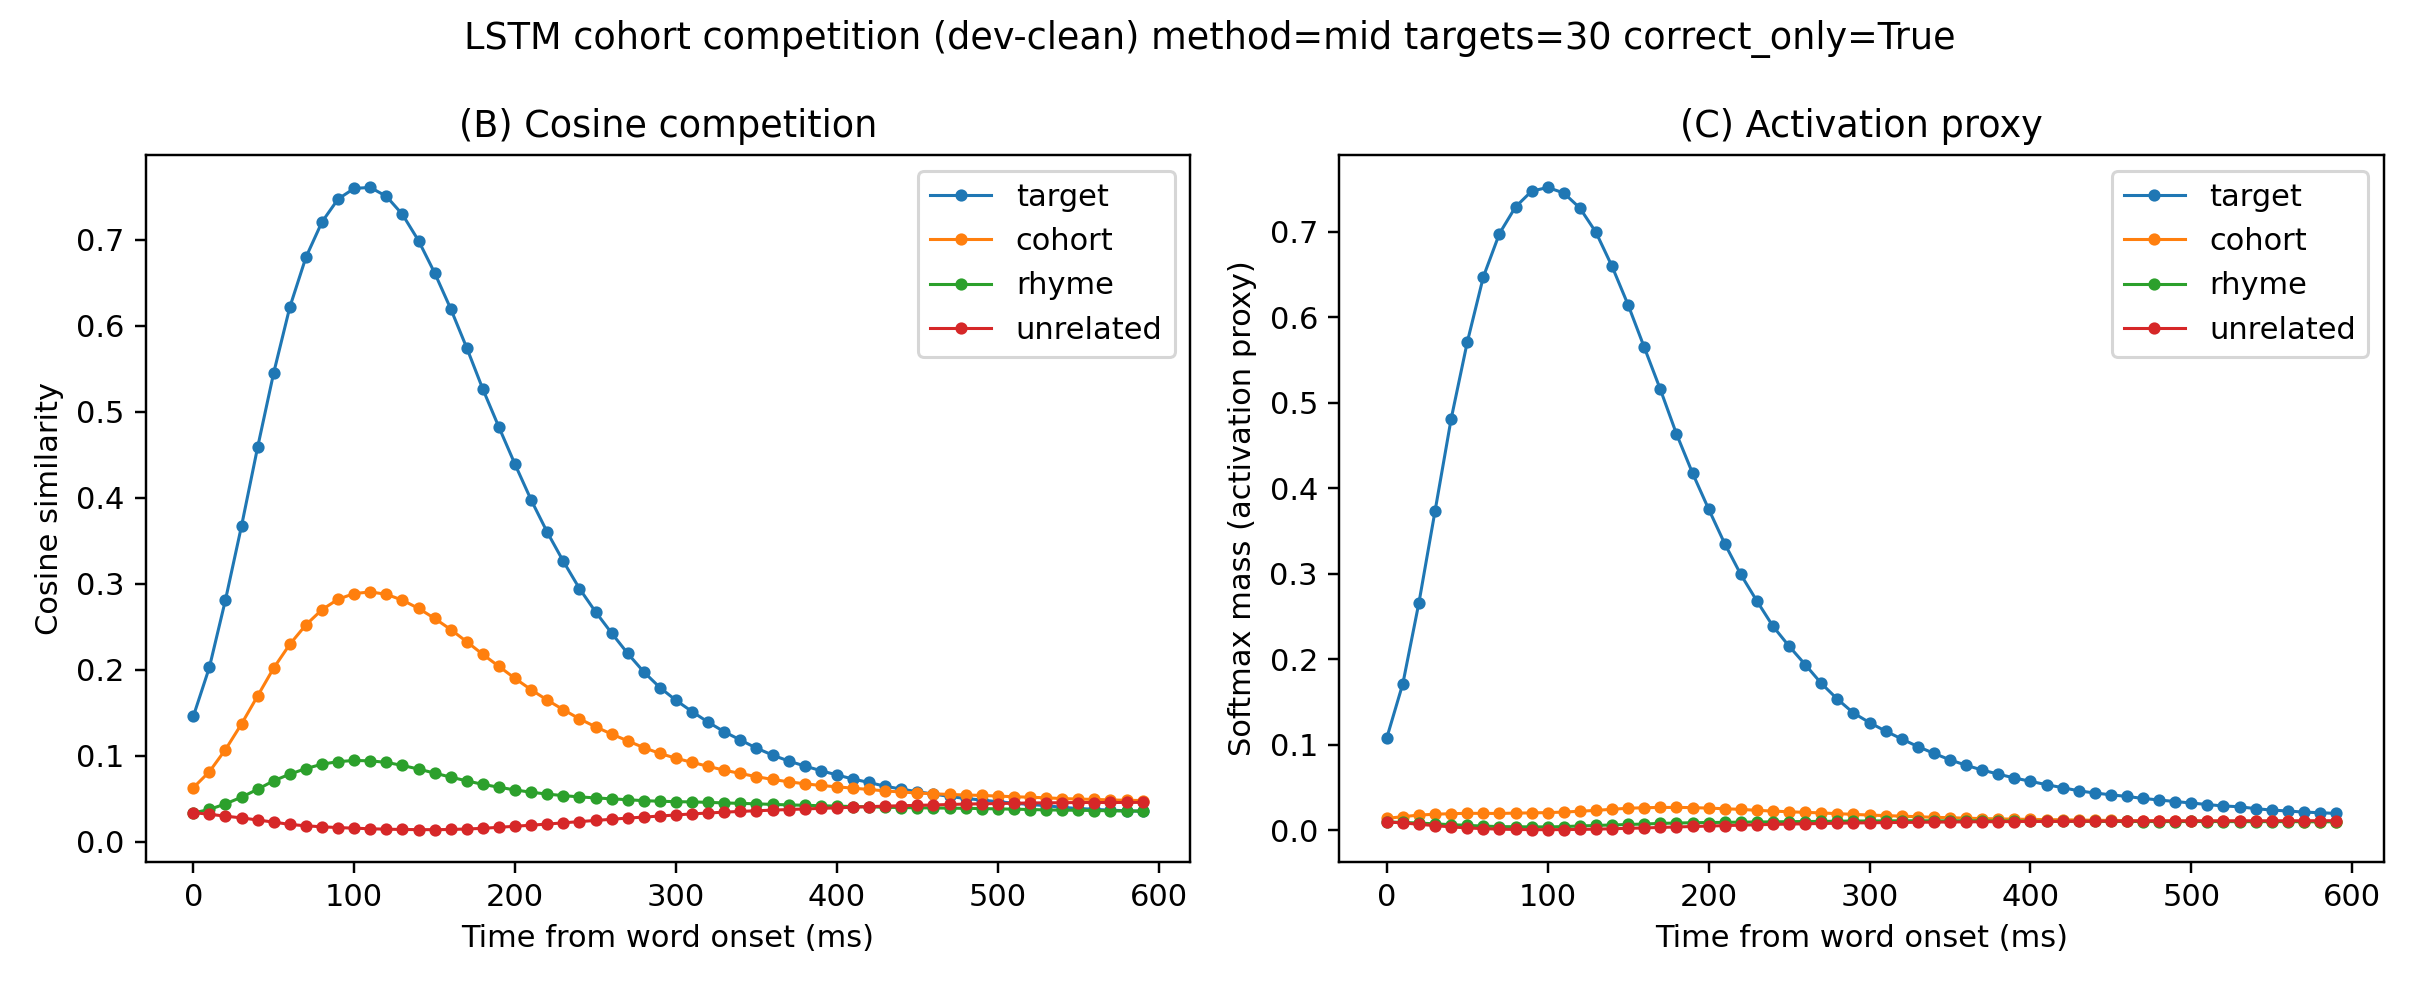
\includegraphics[width=0.9\textwidth]{example.png}
    \caption{Representative output generated by the end-to-end workflow. The figure illustrates that the pipeline can successfully produce analysis results.}
    \label{fig:vnv-performance-example}
\end{figure}

\begin{figure}[ht]
    \centering
    \begin{subfigure}[b]{0.48\textwidth}
        \centering
        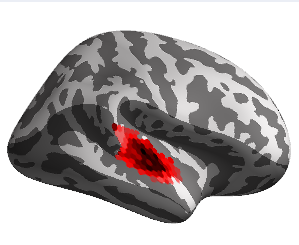
\includegraphics[width=\textwidth]{rh1.png}
        \caption{gt-based brain response result.}
        \label{fig:brain1}
    \end{subfigure}
    \hfill
    \begin{subfigure}[b]{0.48\textwidth}
        \centering
        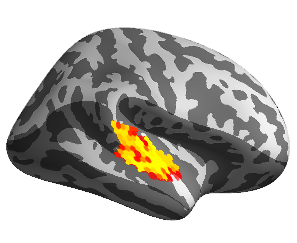
\includegraphics[width=\textwidth]{rh2.png}
        \caption{edge-based brain response result.}
        \label{fig:brain2}
    \end{subfigure}
    \caption{Representative brain visualization outputs generated by the pipeline.}
    \label{fig:brain_pair}
\end{figure}















    
\section{Comparison to Existing Implementation}

The existing implementation used in previous work by Brodbeck et al.~\cite{brodbeck2025recurrent} was primarily designed to evaluate a single recurrent neural network (RNN) model in a specific experimental setting.
That implementation was effective for the original study, but its scope was relatively narrow and extending it to additional model types or predictor variants would require more manual modification.

In contrast, the implementation developed in this project is designed as a more general experimental framework.
Instead of supporting only one recurrent model, it supports multiple deep learning model configurations through a modular structure.
New model architectures can be added by placing the corresponding network implementation in the \texttt{network} directory and adding the required configuration entries in the \texttt{config} module.
This reduces the effort required to evaluate additional model types and makes the framework more suitable for comparative experiments.

Another important difference is that the current implementation organizes the workflow into a more complete pipeline, including model training or loading, predictor extraction, predictor alignment, mTRF fitting, score computation, and summary generation.
This makes it easier to reuse the framework for future experiments and lowers the onboarding cost for new users in the lab.

Overall, compared to the earlier implementation, the current system provides improved extensibility, improved maintainability, and a more unified end-to-end workflow.
However, the present implementation still has some limitations.
For example, cross-platform evaluation is currently incomplete, since the framework has been used extensively on Windows and Linux but has not yet been fully tested on macOS.
Therefore, the current implementation should be understood as a substantial engineering extension of the earlier single-model workflow rather than a complete replacement in all settings.



\section{Unit Testing}

Unit testing was performed using \texttt{pytest}.
The purpose of these tests was to verify the correctness of individual functions, classes, and small modules in isolation, without requiring the full end-to-end pipeline to run.
The unit tests focused on local logic such as parameter validation, configuration generation, checkpoint parsing, protocol consistency checking, and scoring error handling.

The main unit-tested components include the configuration module, the checkpoint loading logic, the predictor protocol validation logic, the predictor alignment checks based on synthetic inputs, and the encoding-score validity checks.
For example, unit tests were used to verify that invalid configuration values are rejected, that predefined training presets generate the expected settings, that model checkpoints in different formats can be parsed correctly, and that invalid scoring inputs such as \texttt{NaN} predictors or constant response signals are detected and reported with appropriate error messages.

Not all implemented tests are strict unit tests.
Some tests written during validation use real datasets, real predictor files, or trained checkpoints, and are therefore better classified as integration tests or data-validation tests rather than pure unit tests.
Examples include tests that check the existence and structure of the Appleseed dataset, the presence of generated predictor files, and the successful loading of real trained checkpoints.
These tests are reported in the functional requirements evaluation and related validation sections rather than being treated as isolated unit tests.

Overall, the unit tests provide evidence that the core local logic of the system behaves correctly under both valid and invalid input conditions, while the higher-level tests provide evidence that the integrated workflow operates correctly on real data. The tests are shown in Table~\ref{tab:unit-test-summary}.


\begin{table}[H]
\centering
\caption{Summary of implemented tests and their classification.}
\label{tab:unit-test-summary}
\begin{tabular}{p{5.0cm} p{3.0cm} p{5.0cm}}
\toprule
\textbf{Test File / Component} & \textbf{Classification} & \textbf{Purpose} \\
\midrule
test\_input\_parameters\_\\module.py & Unit test & Validate enums, schema rules, presets, and configuration utilities \\
test\_model\_ckpt\_\\loading.py & Unit test / Integration test & Verify checkpoint parsing logic; some cases use real checkpoints \\
test\_predictor\_protocol\_\\validation.py\ & Unit test & Detect conflicting predictor protocol fields \\
test\_predictor\_\\alignment.py & Unit test & Verify alignment failure on incompatible synthetic time axes \\
test\_encoding\_score\_\\invalidity.py & Unit test & Verify rejection of invalid scoring inputs \\
test\_encoding\_score\_\\invalidity\_eelbrain.py & Unit test & Verify NDVar-based invalid scoring cases \\
test\_librispeech\_aligned\\\_words\_integration.py & Integration test & Validate dataset reading using real manifest and feature files \\
test\_appleseed\_meg\\\_dataset.py & Integration / data validation test & Validate Appleseed dataset structure and MEG files \\
test\_appleseed\_\\predictors.py & Integration / data validation test & Validate generated predictor pickle files \\
test\_eelbrain\_cached\_\\scores.py & Integration test & Validate cached Eelbrain scoring outputs \\
\bottomrule
\end{tabular}
\end{table}






\section{Changes Due to Testing}

% \wss{This section should highlight how feedback from the users and from 
% the supervisor (when one exists) shaped the final product.  In particular 
% the feedback from the Rev 0 demo to the supervisor (or to potential users) 
% should be highlighted.}


Several changes were made as a result of testing.

First, the LSTM training framework was extended to support multiple loss functions.
This change was introduced so that different loss settings could be tested and compared more easily.
Additional plotting functionality was also added to visualize the cohort-level results under different loss functions.

Second, the mTRF evaluation workflow was extended to support fitting in different brain regions.
In particular, the workflow was updated so that STG and late language regions could be analyzed separately.
This change made the analysis more informative and better aligned with the intended neuroscience use case.

Overall, testing led to improvements in both the deep learning training pipeline and the downstream brain-response evaluation workflow.







\section{Automated Testing}

Automated testing was performed only at the component level.
Several \texttt{pytest}-based tests were written for configuration validation, checkpoint loading, predictor validation, and score error handling.
However, a fully automated end-to-end testing pipeline has not yet been established.

This project is a research framework and depends on large datasets, trained models, Eelbrain analysis steps, and GPU-supported environments.
Because of these dependencies, the main testing priority has been to ensure the correctness of training and analysis in the real research environment rather than to build a complete continuous integration workflow.

Therefore, the current project uses local automated tests for selected modules, while full workflow validation is still performed manually.
Future work may add lightweight CI-based smoke tests for selected parts of the system.



		
\section{Trace to Requirements}

This section provides traceability between the requirements defined in the SRS/VnV Plan and the corresponding tests or evaluation evidence in this report.
Each functional requirement (FR) and nonfunctional requirement (NFR) is linked to the most relevant test file, evaluation subsection, or supporting evidence.
The table is shown in Table~\ref{tab:trace_to_requirements1} and \ref{tab:trace_to_requirements2}.

\begin{table}[h]
\centering
\caption{Traceability between FR and tests/evaluation evidence}
\label{tab:trace_to_requirements1}
\begin{tabularx}{0.96\textwidth}{p{2.0cm}X}
\toprule
\textbf{FR} & \textbf{Tests / Evaluation Evidence} \\
\midrule

FR-01 & \texttt{test\_appleseed\_meg\_dataset.py} (MEG dataset structure validation). This provides partial coverage for MEG metadata/path validation, but a dedicated invalid-\texttt{fs} test should be added if strict one-to-one coverage of FR-01 is required. \\

FR-02 & \texttt{test\_input\_parameters\_module.py} (invalid/unsupported configuration values and preset validation). \\

FR-03 & \texttt{test\_input\_parameters\_module.py} (invalid numeric ranges and configuration constraint checks for model hyperparameters). \\

FR-04 & \texttt{test\_model\_ckpt\_loading.py} and synthetic forward-pass checks. This provides partial coverage for model input compatibility, but a dedicated feature-dimension mismatch test should be added for exact FR-04 coverage. \\

FR-05 & \texttt{test\_librispeech\_aligned\_words\_unit.py}, \texttt{test\_librispeech\_aligned\_words\_integration.py} (manifest loading, missing feature file handling, and dataset validation). \\

FR-06 & \texttt{test\_predictor\_alignment.py} (synthetic incompatible predictor/MEG time-axis alignment failure). \\

FR-07 & \texttt{test\_predictor\_protocol\_validation.py} (conflicting predictor evaluation protocol fields). \\

FR-08 & \texttt{test\_encoding\_score\_invalidity.py}, \texttt{test\_encoding\_score\_invalidity\_eelbrain.py}, \texttt{test\_eelbrain\_cached\_scores.py} (invalid scoring inputs and invalid cached score detection). \\


\bottomrule
\end{tabularx}
\end{table}




\begin{table}[H]
\centering
\caption{Traceability between NFR and tests/evaluation evidence}
\label{tab:trace_to_requirements2}
\begin{tabularx}{0.96\textwidth}{p{2.0cm}X}
\toprule
\textbf{NFR} & \textbf{Tests / Evaluation Evidence} \\
\midrule


NFR-01 & Nonfunctional Requirements Evaluation: Usability; in-class end-to-end demonstration, face-to-face feedback from users familiar with Eelbrain, and discussion feedback from Professor Brodbeck. \\

NFR-02 & Nonfunctional Requirements Evaluation: Maintainability; modular \texttt{network} and \texttt{config} structure, and low-effort extension evidence for adding new model settings. \\

NFR-03 & Nonfunctional Requirements Evaluation: Portability; successful execution evidence on Windows and Linux, with macOS not yet completed. \\

NFR-04 & Nonfunctional Requirements Evaluation: Reproducibility; repeated-run comparison table and associated logs/results. \\

NFR-05 & Nonfunctional Requirements Evaluation: Performance; benchmark summary table, timing logs, and representative generated artifacts/figures. \\

\bottomrule
\end{tabularx}
\end{table}



		
\section{Trace to Modules}

This section provides traceability between the modules defined in the MIS and the corresponding tests or evaluation evidence in this report.
Each module is linked to the most relevant unit tests, integration tests, or evaluation subsections.
The purpose of this section is to show that all major modules of \progname{} have been covered by verification and validation activities.
The table is shown in Table~\ref{tab:trace_to_modules}.


\begin{table}[H]
\centering
\caption{Traceability between modules and tests}
\label{tab:trace_to_modules}
\begin{tabularx}{0.96\textwidth}{p{3.6cm}X}
\toprule
\textbf{Module} & \textbf{Tests / Evidence} \\
\midrule
\textbf{M1 Audio Data Module} & \texttt{test\_librispeech\_aligned\_words\_unit.py}, \texttt{test\_librispeech\_aligned\_words\_integration.py} \\
\textbf{M2 MEG Data Module} & \texttt{test\_appleseed\_meg\_dataset.py} \\
\textbf{M3 Input Parameters Module} & \texttt{test\_input\_parameters\_module.py} \\
\textbf{M4 Model Training Module} & configuration validation tests; reproducibility/performance evaluation \\
\textbf{M5 Frozen Model Module} & \texttt{test\_model\_ckpt\_loading.py} \\
\textbf{M6 Representation Extraction Module} & \texttt{test\_appleseed\_predictors.py}, \texttt{test\_predictor\_alignment.py} \\
\textbf{M7 Statistical Analysis Module} & \texttt{test\_predictor\_protocol\_validation.py}, \texttt{test\_encoding\_score\_invalidity.py}, \texttt{test\_encoding\_score\_invalidity\_eelbrain.py}, \texttt{test\_eelbrain\_cached\_scores.py} \\
\textbf{M8 Plotting Module} & generated output figures; plotting changes described in Changes Due to Testing \\
\bottomrule
\end{tabularx}
\end{table}






\section{Code Coverage Metrics}

Code coverage metrics were not collected systematically for this project.
In particular, no formal statement coverage or branch coverage report was generated during development.

The main reason is that \progname{} is a research framework rather than a conventional software product.
At the current stage, the primary testing goal has been to ensure the correctness of data processing, model training or loading, predictor generation, statistical analysis, and final result interpretation.
As a result, testing effort has focused on functional validation and selected automated \texttt{pytest}-based checks rather than on maximizing code coverage metrics.

In addition, several important parts of the framework depend on large datasets, trained checkpoints, Eelbrain analysis objects, and research-specific execution environments.
For this reason, numerical correctness and end-to-end workflow validity were considered more important than obtaining a high code coverage percentage.

Although formal coverage metrics are not currently available, the project does include tests for several important components, including configuration validation, checkpoint loading, predictor validation, alignment checks, and invalid scoring conditions.
Future work may add coverage tools to quantify which parts of the codebase are exercised by the current automated tests.


% \section{Extras}

% \wss{Summary of the status of your extras.  If feasible, the extras should be
% complete by the time of writing the VnV report.  If the extras are not complete,
% you should summarize the plans for completing them.}

\bibliographystyle{plainnat}
\bibliography{../../refs/References}

\newpage{}
\section*{Appendix --- Reflection}

The information in this section will be used to evaluate the team members on the
graduate attribute of Reflection.

\input{../Reflection.text}

\begin{enumerate}
  \item \textbf{What went well while writing this deliverable?}

  
  First, the structure of the project itself was relatively modular, which made it easier to map the implementation to the VnV Report.


  Second, many important test cases had already been explored during development, even if they were not originally written in the exact format required for the VnV deliverable.
  This made it possible to convert existing checks into formal test cases for functional requirements.


  Third, the deliverable also benefited from the fact that the framework had already been used to run real experiments and generate actual results and figures.
  This made the nonfunctional evaluation more concrete, since usability, maintainability, performance, and practical usefulness could all be discussed with real evidence rather than only hypothetical claims.

  \item \textbf{What pain points did you experience during this deliverable, and how did you resolve them?}

  The main pain point was that this project is a research framework rather than a conventional software product.
  As a result, many parts of the system depend on large datasets, trained checkpoints, Eelbrain analysis objects, and GPU-supported environments.
  This made it difficult to fit all validation activities into the standard software engineering categories such as pure unit testing, code coverage, or fully automated CI testing.

  Another difficulty was distinguishing between different types of tests.
  Some of the implemented tests were true unit tests, such as configuration validation or synthetic invalid-scoring checks, while others were closer to integration or data-validation tests, such as checking the Appleseed dataset structure or loading real predictor files.




  \item \textbf{Which parts of this document stemmed from speaking to your client(s) or a proxy (e.g. your peers)? Which ones were not, and why?}

  Several parts of the document were informed directly by discussions with the client or proxies.
  The usability evaluation was strongly influenced by classroom demonstration and face-to-face discussions with peers who are familiar with Eelbrain, especially Lizhangwenchi and Yanyu.
  Their feedback helped support the claim that the workflow was easy to understand and operate.
  In addition, discussion with Professor Brodbeck helped shape the assessment of the framework's practical usefulness.
  In particular, the idea that this framework could reduce onboarding cost for future students in the lab directly influenced the usability and maintainability discussion.

  The emphasis on separating STG from later language-related regions in the mTRF workflow was also closely related to the intended neuroscience use case, which was clarified through domain discussions rather than derived only from software structure.



  \item \textbf{In what ways was the Verification and Validation (VnV) Plan different from the activities that were actually conducted for VnV? If there were differences, what changes required the modification in the plan? Why did these changes occur? Would you be able to anticipate these changes in future projects?}


  The main difference was that the plan was written in a more idealized and requirement-driven style, while the actual validation work had to adapt to the realities of a research environment.
  In the plan, many requirements were described as if they would each be validated by a dedicated and isolated test.
  In practice, the implemented testing combined several styles: synthetic \texttt{pytest} tests for invalid cases, local automated checks for important functions, manual evaluation for usability-related aspects, and evidence from real experimental runs for performance and practical usefulness.

  Another difference was that the original plan suggested more complete automated workflows, including stronger portability and reproducibility evaluation.
  In practice, the project was used extensively on Windows and Linux, but not yet fully tested on macOS.
  Similarly, local automated tests were written, but a full CI-based automated testing pipeline and systematic code coverage metrics were not implemented.
  These differences occurred because the framework depends on large datasets, trained deep learning models, Eelbrain objects, and environment-specific resources such as GPUs and local file paths.
  Under these constraints, ensuring the correctness of training, predictor generation, and analysis outputs was more important than implementing a fully automated software-engineering pipeline.

  The actual testing activities also led to engineering changes that were not fully anticipated at the planning stage.
  For example, testing motivated extending the LSTM training framework to support multiple loss functions and adding plots to compare cohort-level results under different losses.
  Testing also motivated extending the mTRF workflow to support fitting in different brain regions, especially distinguishing STG from later language-related areas.
  These changes were driven by the fact that validation revealed practical scientific needs that were not fully obvious when the original plan was written.

  In future projects, some of these differences could be anticipated earlier.
  In particular, it would be helpful to explicitly separate three categories from the beginning.
  It would also be useful to plan lightweight CI tests only for synthetic or small-scale cases, while keeping full experimental validation as a separate activity.
  However, some deviation would probably still be unavoidable in research software, because scientific goals often evolve as the system is tested on real data and real analyses.
\end{enumerate}

\end{document}